\chapter{La détection d'anomalies en Spark/Scala} \label{application:spark}

Nous avons utilisé plusieurs classes, notées case class en langage Scala. Ces classes permettent de modéliser les données tout au long du processus de l'analyse des traceroutes. 
Nous présentons les différentes case class créées au fur et au mesure de leur utilisation.


\section{Les case class }

\paragraph{La classe Signal} modélise un signal \footnote{Un signal dans le contexte d'un traceroute.}. Ainsi, \textit{from} est l'adresse IP du routeur émettant ce signal, \textit{rtt} est le Round Trip Time entre la sonde Atlas et ce routeur et enfin \textit{x} est un indicateur de l'échec du signal.
\begin{lstlisting}[language=scala, caption={La classe Signal en Scala }]
case class Signal(
	rtt:  Option[Double],
	x:    Option[String],
	from: Option[String])

\end{lstlisting}

\paragraph{La classe Hop} modélise un saut dans un traceroute. On caractérise un saut par son identifiant noté \textit{hop}. Celui-ci   prend comme valeur un entier commençant à $1$ et la liste des signaux relatifs à ce saut, appelée  \textit{result}. Généralement un saut est représenté par $3$ signaux.
\begin{lstlisting}[language=scala, caption={La classe Hop en Scala }]
case class Hop(
	var result: Seq[Signal],
	hop:        Int)
\end{lstlisting}
\paragraph{La classe Traceroutes} modélise le résultat d'une requête traceroute effectuée par une sonde Atlas. Cette modélisation se limite aux données qui nous intéressent dans la présente analyse : 
\textit{dst\_name} représente l'adresse IP de la destination de la requête traceroute, \textit{from} est l'adresse IP de la sonde, \textit{prb\_id} est l'identifiant de la sonde, \textit{msm\_id} est l'identifiant de mesure, \textit{timestamp} est le temps auquel la requête traceroute a été effectuée et enfin on trouve la liste des sauts qui représentent les routeurs traversés par le trafic entre la source et la destination. 

\begin{lstlisting}[language=scala, caption={La classe Traceroute en Scala }]
case class Traceroute(
	dst_name:  String,
	from:      String,
	prb_id:    BigInt,
	msm_id:    BigInt,
	timestamp: BigInt,
	result:    Seq[Hop])
\end{lstlisting}
\paragraph{La classe TraceroutesPerPeriod} permet de présenter les traceroutes après les avoir regroupé    suivant la période pendant laquelle ils ont été effectués.   \textit{timeWindow} est le temps unix marquant le début de la période \footnote{Pour précision, la fin de la période peut être inférée en prenant deux débuts de deux périodes consécutives car la durée d'une période est fixe tout au long de l'analyse.} et  \textit{traceroutes} est la liste des traceroutes effectués pendant cette période. 


A l'étape 2, l'objectif était d'agréger  les signaux par routeur source et ensuite calculer la médiane des RTTs par ce routeur. Par conséquent, un traceroute est présenté différemment, ce qui est  illustré par la classe \textit{MedianByHopTraceroute}.

\paragraph{La classe PreparedSignal }  est une agrégation de tous les signaux, d'un saut donné, par le routeur \textit{from},  la médiane des RTTs calculée est présentée par \textit{medianRtt}.
\begin{lstlisting}[language=scala, caption={La classe PreparedSignal en Scala }]
case class PreparedSignal(
	medianRtt: Double,
	from:      String)
\end{lstlisting}
\paragraph{La classe PreparedHop } modélise un saut après avoir agrégé ses signaux. 
\begin{lstlisting}[language=scala, caption={La classe PreparedHop en Scala }]
case class PreparedHop(
	var result: Seq[PreparedSignal],
	hop:        Int)
\end{lstlisting}


\paragraph{La classe MedianByHopTraceroute } modélise un traceroute après avoir agrégé ses sauts. Par rapport au traceroute d'avant l'agrégation, seule la liste des sauts  a subi un changement. 
\begin{lstlisting}[language=scala, caption={La classe MedianByHopTraceroute en Scala }]
case class MedianByHopTraceroute(
	dst_name:  String,
	from:      String,
	prb_id:    BigInt,
	msm_id:    BigInt,
	timestamp: BigInt,
	result:    Seq[PreparedHop])
\end{lstlisting}


\paragraph{La classe Link} modélise un lien topologique. Ce dernier est défini par deux adresses IP  \textit{ip1} et \textit{ip2} et par son RTT différentiel calculé \textit{rttDiff}.
\begin{lstlisting}[language=scala, caption={La classe Link en Scala }]
case class Link(
	ip1:     String,
	ip2:     String,
	rttDiff: Double)
\end{lstlisting}

\paragraph{La classe LinksTraceroute} permet de modéliser un traceroute après avoir inféré tous ses liens. Ainsi, la liste des sauts est remplacée par la liste des liens (\textit{links}). 

\begin{lstlisting}[language=scala, caption={La classe LinksTraceroute en Scala }]
case class LinksTraceroute(
	dst_name:  String,
	from:      String,
	prb_id:    BigInt,
	msm_id:    BigInt,
	timestamp: BigInt,
	links:     Seq[Link])
\end{lstlisting}


A l'étape $5$, l'objectif est de passer d'un traceroute à une liste de liens caractérisés par les informations générales de la requête traceroute et leurs RTTs différentiels. Chaque élément de cette liste est représenté par la classe \textit{DiffRtt}, où \textit{LinkIPs} représente les deux adresses IP d'un lien donné.
\paragraph{La classe LinkIPs} permet représenter un lien par seulement ses deux adresses IP \textit{ip1} et \textit{ip2}.
\begin{lstlisting}[language=scala, caption={La classe LinkIPs en Scala }]
case class LinkIPs(
	ip1: String,
	ip2: String)
\end{lstlisting}

\paragraph{La classe DiffRtt} est une représentation plus détaillée d'un lien, en plus de son RTT différentiel, on ajoute d'autres informations.  Les adresses IP d'un lien sont modélisées par la classe \textit{LinkIPs}.

\begin{lstlisting}[language=scala, caption={La classe DiffRtt en Scala }]
case class DiffRtt(
	rtt:      Double,
	var link: LinkIPs,
	probe:    BigInt)
\end{lstlisting}

A l'étape $6.2$, on souhaite normaliser les dates de chaque lien; peu importe le moment pendant lequel le traceroute a été effectué durant une période $d_k$, on note seulement le début de cette période. Ainsi,  la classe  \textit{DiffRTTPeriod}  reprend un \textit{lien} donné, les différentes sondes Atlas ayant identifié ce lien (\textit{probes}), les RTTs différentiels de ce lien tout au long de cette période (\textit{rtts}) et enfin les dates associées à chaque RTT différentiel (\textit{dates}).
\paragraph{La classe DiffRTTPeriod } ~
\begin{lstlisting}[language=scala, caption={La classe DiffRTTPeriod en Scala }]
case class DiffRTTPeriod(
	link:      LinkIPs,
	probes:    Seq[BigInt],
	rtts:      Seq[Double],
	var dates: Seq[Int])
\end{lstlisting}

A la fin des opérations de l'étape $6$, on reprend pour chaque période, pour un lien donné, les RTTs différentiels ainsi que leurs dates. Ensuite, on calcule les bornes de l'intervalle de confiance courant pour ce lien et les bornes de l'intervalle de confiance de référence, et ce afin de comparer ces deux intervalles en vue d'inférer les anomalies possibles du délais de ce lien. Les intervalles de confiance sont calculés à en utilisant  la méthode des scores de Wilson.


\paragraph{La classe LinkState } permet de modéliser les intervalles de confiance d'un lien pendant une période $d_k$ donnée. \textit{valueLow} est la borne inférieur de l'intervalle de confiance, \textit{valueHi} est la borne supérieure de l'intervalle de confiance, \textit{valueMedian} est la médiane des RTTs différentiels et enfin \textit{valueMean} est la moyenne des RTTs différentiels. Pour précision, les données concernant l'état d'un lien sont sous forme d'une liste. L'idée est de garder l'historique de ces valeurs durant toute la période de l'analyse. Cette historique est exploitée pour tracer l'évolution du RTT différentiel du lien. Cependant, la comparaison utilise les valeurs du dernier état du lien.

  

%Pour toute période, on a une instance de \textit{LinkState} pour 
\begin{lstlisting}[language=scala, caption={La classe LinkState en Scala }]
case class LinkState(
	var valueMedian: Seq[Double],
	var valueHi:     Seq[Double],
	var valueLow:    Seq[Double],
	var valueMean:   Seq[Double])
\end{lstlisting}

Nous avons décrit les différentes classes utilisées. En ce qui concerne les traitements à appliquer sur les données, ce sont les fonctions permettant de répondre aux détails des étapes décrites dans la section  \ref{steps-rtt-analysis}.


\section{Processus}

\paragraph{Exécution d'une application Spark} Afin de pouvoir exécuter une application Spark, il faut qu'elle soit packagée dans un fichier de type JAR. Ce dernier doit reprendre une classe contenant une méthode \textit{main} et doit reprendre toutes les dépendances nécessaires à l'exécution de l'application. Nous avons utilisé \textit{Maven}\footnote{\url{https://maven.apache.org/}, consultée le $09/04/2019$.} pour automatiser la gestion du fichier JAR. Enfin, l'application Spark  est soumise avec la commande \textit{bin/spark-submit}. Un exemple d'une soumission est donné dans \ref{lst:submit}.

\begin{lstlisting}[language=bash,firstnumber=1, caption={Exemple de la soumissions d'un traitement sur Spark},label={lst:submit}, basicstyle = \small,escapechar=|,numbers=left,
stepnumber=1]
~$ bin/spark-submit --class ripeatlasanalysis.AnalyseTraceroute     --master local --driver-memory 30G  --conf "spark.network.timeout=10000000" SparkExample-lowprints-0.0.5-SNAPSHOT-jar-with-dependencies.jar  1517961600  1518134400 3600 
\end{lstlisting}
La commande \textit{bin/spark-submit} prend plusieurs paramètres, nous présentons quelques paramètres utilisés :
\begin{itemize}
	\item \textit{class} est un objet Scala contenant la fonction \textit{main};
	\item  \textit{master} est l'URL du cluster. Par exemple la valeur \textit{local} indique que Spark est exécuté localement avec un seul worker thread (aucun parallélisme), alors que \textit{local[K]} lance le traitement sur Spark en utilisant $K$ worker sur $K$ threads, idéalement $K$ est le nombre des  c\oe{}urs de la machine;
	\item \textit{driver-memory} est la mémoire dont le processus du driver peut utiliser;
	
	\item  \textit{--conf} "key = value" est une manière de configurer l'application Spark. Dans l'exemple, "spark.network.timeout=10000000", $ 10000000 $ est le temps durant lequel le driver doit recevoir  des mises à jour de la part des différents workers; après ce temps, le worker n'est plus considéré comme actif.
\end{itemize}

\paragraph{Configuration d'une application  Spark}

Une application Spark nécessite l'ajustement de quelques paramètres, qu'il s'agit d'une application qui tourne en mode local ou bien en mode cluster. Il est possible de passer certains paramètres selon trois possibilités. D'abord, dans l'objet \textit{SparkConf} comme illustré dans l'exemple ci-dessous où nous donnons un nom à l'application Spark (ligne \ref{line:app-name} Listing \ref{lst:label}) et nous précisons le nombre de threads à créer (ligne \ref{line:app-thread} Listing \ref{lst:label}). 

\begin{lstlisting}[language=scala,firstnumber=1, caption={Exemple de configuration avec SparkConf},label={lst:label}, basicstyle = \footnotesize,escapechar=|,numbers=left,
stepnumber=1]
//imports
import org.apache.spark.SparkConf

// Spark configuration : create configuration
val conf = new SparkConf().setAppName("RTT delays analysis") |\label{line:app-name}|
                          .setMaster("local"),  |\label{line:app-thread}|
\end{lstlisting}

Certains paramètres peuvent être précisés 

%en ligne de commande ou bien dans le fichier de configuration \footnote{Plus de détails sont disponibles.}. 
%La configuration de l'application s'effectue à travers un . Il existe un nombre de  paramètres à  ajuster comme le nombre de threads à utiliser au cas où l'application Spark s'exécute en mode local.



\paragraph{Point d'entrée vers les fonctionnalités du Spark}

Le point d'entrée vers les fonctionnalités du Spark se fait par la création du  \textit{SparkContext}. Toutefois, il existe d'autre points d'entrée plus spécifique aux composantes du \textit{Spark Uniffied Stack}. Par exemple,  \textit{SparkSession} est le point d'entrée vers Spark SQL, StreamingContext est le point d'entrée vers Spark Streaming, etc.


\paragraph{Les paramètres de l'analyse}

Afin de tracer l'évolution du délai des liens, nous avons besoin des traceroutes stockés dans objets JSON, la date du début de l'analyse ($ 1517961600 $), la date de fin ($ 1518134400 $) et enfin la durée de la période ($3600$s). En ce qui concerne les fichiers de données, ils sont stockés localement et le chemin vers ces derniers est configuré dans un fichier de configuration.


\paragraph{La lecture des données}

L'outil de détection proposé par R. Fontugne et al. n'exploite qu'une partie des données d'une réponse traceroute \footnote{Voir un exemple d'une réponse  traceroute  dans \ref{exemple-traceroute}.}. 
En particulier, Spark offre la possibilité de ne lire que les données qui nous intéressent\footnote{C'est le principe du Schema-On-Read décrit dans \ref{sec:schema-read-write}.}. 

Chaque réponse traceroute est structurée dans un objet JSON et par ligne. Afin de lire chaque ligne, nous avons créé une case class qui a pour objectif de faire l'association entre l'objet JSON  et un objet Traceroute. Une classe \textit{Traceroute} reprend le nom de la destination de la requête traceroute (\textit{dst\_name}), l'adresse IP de la sonde effectuant la requête traceroute (\textit{from}), l'identifiant de la sonde (\textit{prb\_id}), le temps de la requête (\textit{timestamp}) et enfin la liste des sauts(\textit{Seq[Hop]}).


\begin{lstlisting}[language=scala,firstnumber=1, caption={Description du case class Traceroute},label={lst:case-class-Traceroute}, basicstyle = \footnotesize,escapechar=|,numbers=left,
stepnumber=1]
case class Traceroute(
	dst_name:  String,
	from:      String,
	prb_id:    BigInt,
	msm_id:    BigInt,
	timestamp: BigInt,
	result:    Seq[Hop])
\end{lstlisting}

Un saut (\textit{Hop})  est défini par son rang (\textit{hop}), ce dernier indique l'ordre du saut en question. Etant donné que la sonde reçoit trois\footnote{Dans certains cas, le nombre de signaux dépasse trois.} signaux de chaque saut, un saut est donc défini par un ensemble de signaux (\textit{Seq[Signal]}).
\begin{lstlisting}[language=scala,firstnumber=1, caption={Description du case class Hop},label={lst:case-class-hop}, basicstyle = \footnotesize,escapechar=|,numbers=left,
stepnumber=1]
case class Hop(
	var result: Seq[Signal],
	hop:        Int)
\end{lstlisting}

Un signal \textit{Signal} est émit par  un routeur  dont l'adresse IP est \textit{from}. Le temps nécessaire à la réception du signal est de  \textit{rtt}. Enfin, \textit{x} est un indicateur de la validité du signal, il se peut que la sonde ne reçoive pas une réponse d'un ou de plusieurs routeurs. 

\begin{lstlisting}[language=scala,firstnumber=1, caption={Description du case class Signal}, label={lst:case-class-hop}, basicstyle = \footnotesize,escapechar=|,numbers=left,
stepnumber=1]
case class Signal(
	rtt:  Option[Double],
	x:    Option[String],
	from: Option[String])
\end{lstlisting}

Maintenant que la classe Traceroute est conçu, nous pouvons passer l'étape de lecture des données. Pour ce faire, utilisons la fonction \textit{read()} via l'objet spark de type SparkSession. Nous spécifions à la méthode le schéma de lecture à travers la classe Traceroute, le chemin vers les fichiers de données (\textit{dataPath}) et comment elles sont structurées les données (\textit{json})
\begin{lstlisting}[language=scala,firstnumber=1, caption={Le mapping entre données et cas class},label={lst:mapping}, basicstyle = \footnotesize,escapechar=|,numbers=left,
stepnumber=1]
val rawTraceroutes = spark.read
	.schema(Encoders.product[Traceroute].schema)
	.json(dataPath)
	.as[Traceroute]
import spark.implicits._ |\label{lst:implicits}|
 \end{lstlisting}

Nous obtenons la liste des objets JSON dans la variable \textit{rawTraceroutes}. Ce dernier est un Dataset d'objets  Traceroute. A la ligne \ref{lst:implicits} du Listing \ref{lst:mapping}, nous appelons certaines fonctionnalités nécessaire à la lecture des données. Il est important de noter que Apache Spark adopte ce qu'on appelle \textit{lazy evaluation}. Ainsi, l'évaluation des différentes transformations ne s'effectuent qu'au moment du déclenchement d'une action sur le résultat de cette transformation.

Tous d'abord, nous devons trouver les périodes entre la date de début et la date de fin (étape FindBins()  (I.1)).  Ensuite, nous cherchons les traceroutes capturés durant ces périodes. 
Dans le travail de référence, et comme les données sont stockées sur des collections MongoDB, le groupement des traceroutes par période se base sur la structuration des noms des collections\footnote{Voir la section \ref{mongodb-impleme}.}. Pour une période donnée, seulement les collections concernées qui seront interrogées.

\begin{lstlisting}[language=scala,firstnumber=1, caption={étape FindBins()  (I.1)},label={lst:findbins}, basicstyle = \small,escapechar=|,numbers=left,
stepnumber=1]
//Generate the start of all  bins : between start date and end date espaced by the timewindow
val rangeDates = generateDateSample(start, end, timewindow)

// Find the start and the end of each bin
val rangeDatesTimewindows = rangeDates.map(f => (f, f + timewindow))
\end{lstlisting}

A cette étape, toutes les périodes ont été déterminées. Nous passons à l'étape du groupement du traceroutes disponibles à l'analyse par période (étape I.2). Nous résumons dans la Figure \ref{fig:read-data-from-mongodb} le groupement des traceroutes comme il est implémenté dans le travail de référence; à chaque période, les traceroutes sont sélectionnés de la base de données MongoDB en se basant sur les noms des collections. 
\begin{figure}[h]
	\centering
	
	\captionsetup{justification=centering}
	\resizebox{\textwidth}{!}{
	% Graphic for TeX using PGF
% Title: /home/hayat/RipeAtlasTraceroutesAnalysis/2019/Rapport_Mai/illustrations/read-data-from-mongodb.dia
% Creator: Dia v0.97+git
% CreationDate: Thu May  9 00:13:02 2019
% For: hayat
% \usepackage{tikz}
% The following commands are not supported in PSTricks at present
% We define them conditionally, so when they are implemented,
% this pgf file will use them.
\ifx\du\undefined
  \newlength{\du}
\fi
\setlength{\du}{15\unitlength}
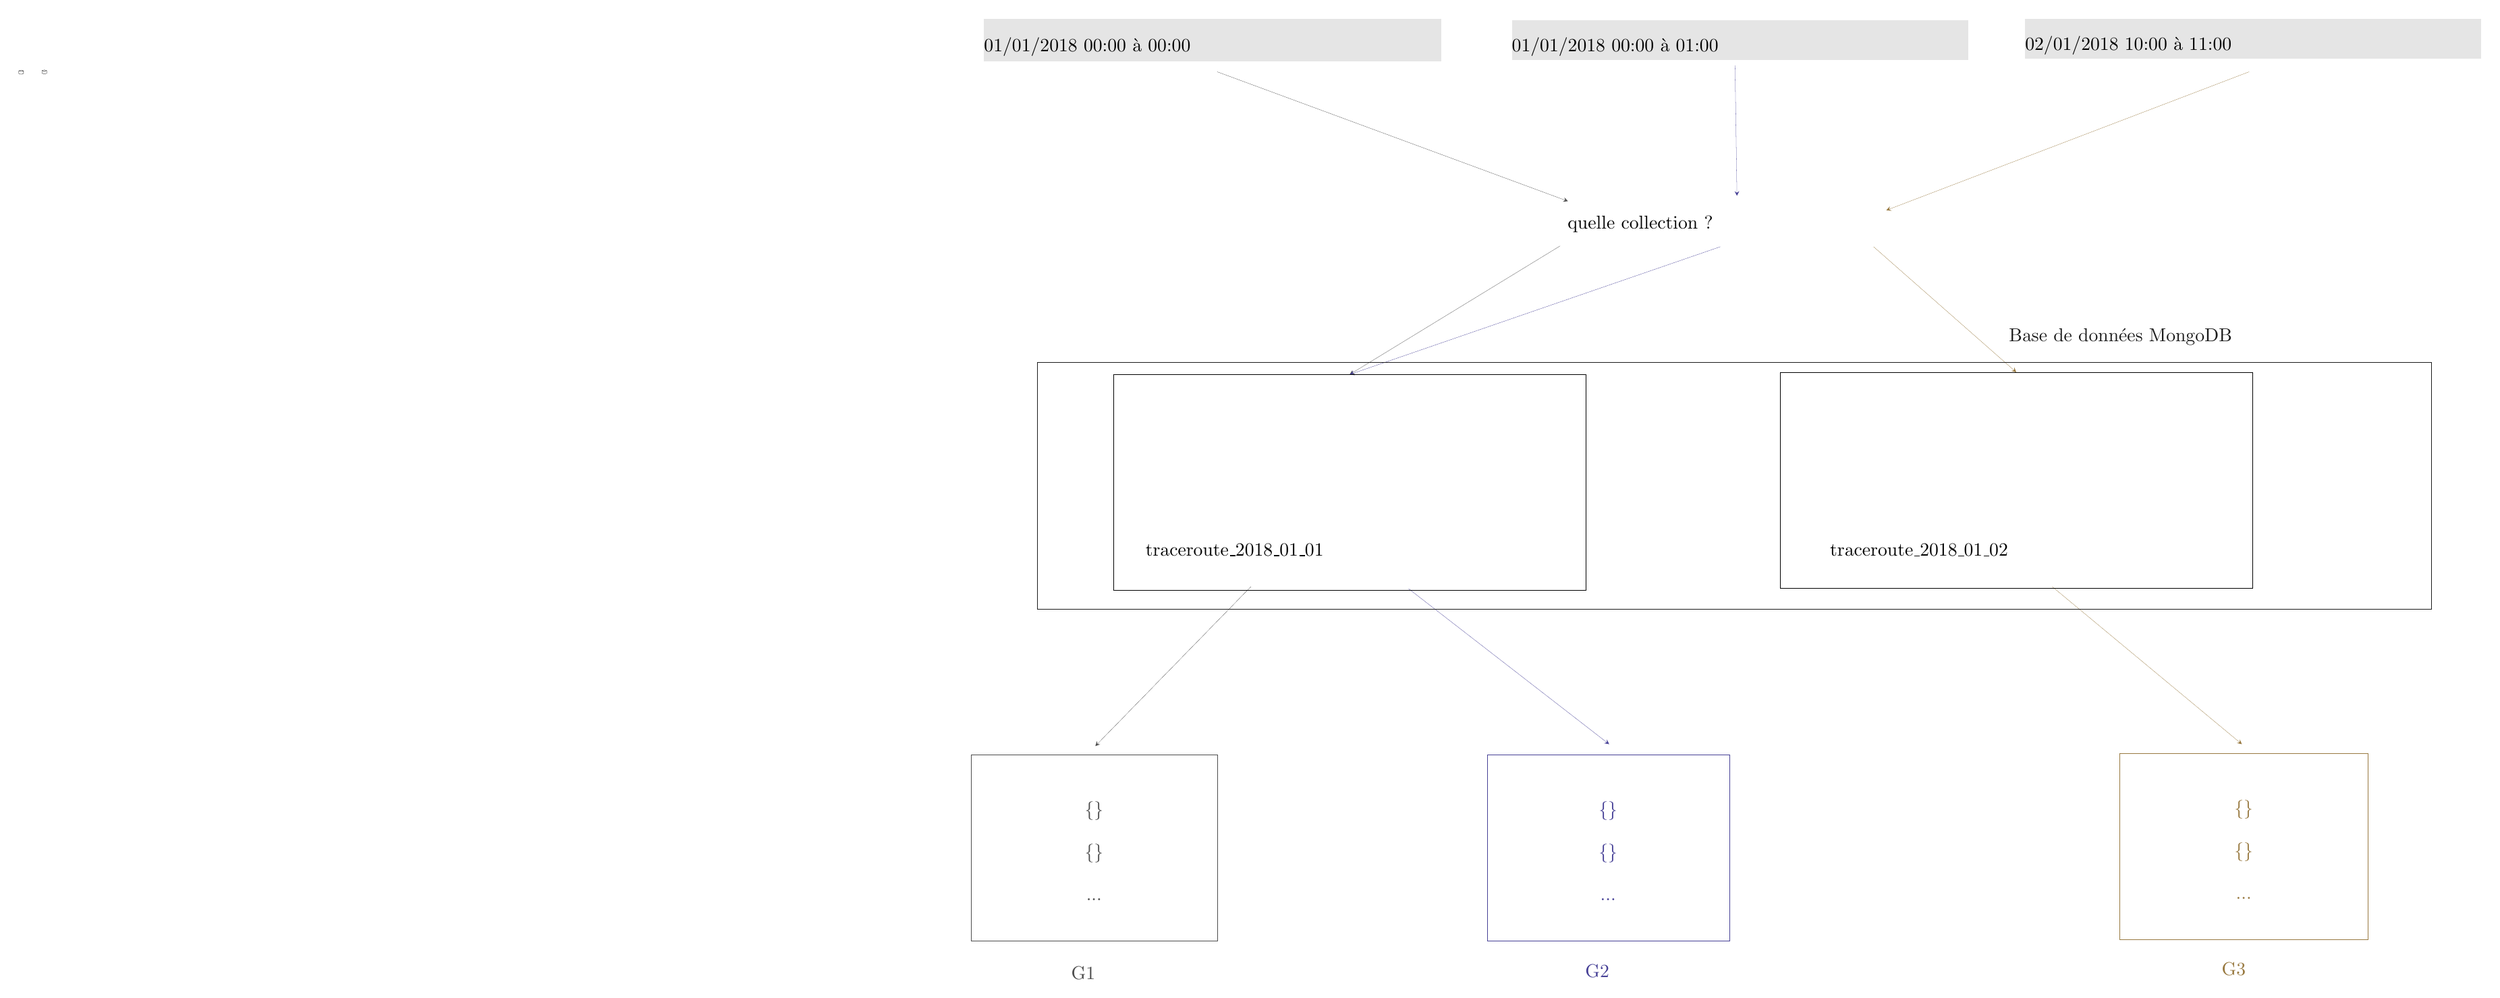
\begin{tikzpicture}[even odd rule]
\pgftransformxscale{1.000000}
\pgftransformyscale{-1.000000}
\definecolor{dialinecolor}{rgb}{0.000000, 0.000000, 0.000000}
\pgfsetstrokecolor{dialinecolor}
\pgfsetstrokeopacity{1.000000}
\definecolor{diafillcolor}{rgb}{1.000000, 1.000000, 1.000000}
\pgfsetfillcolor{diafillcolor}
\pgfsetfillopacity{1.000000}
% setfont left to latex
\definecolor{dialinecolor}{rgb}{0.000000, 0.000000, 0.000000}
\pgfsetstrokecolor{dialinecolor}
\pgfsetstrokeopacity{1.000000}
\definecolor{diafillcolor}{rgb}{0.000000, 0.000000, 0.000000}
\pgfsetfillcolor{diafillcolor}
\pgfsetfillopacity{1.000000}
\node[anchor=base west,inner sep=0pt,outer sep=0pt,color=dialinecolor] at (22.068100\du,9.377600\du){traceroute\_2018\_01\_01};
\pgfsetlinewidth{0.100000\du}
\pgfsetdash{}{0pt}
\pgfsetbuttcap
\pgfsetmiterjoin
\pgfsetlinewidth{0.100000\du}
\pgfsetbuttcap
\pgfsetmiterjoin
\pgfsetdash{}{0pt}
\definecolor{diafillcolor}{rgb}{1.000000, 1.000000, 1.000000}
\pgfsetfillcolor{diafillcolor}
\pgfsetfillopacity{1.000000}
\definecolor{dialinecolor}{rgb}{0.000000, 0.000000, 0.000000}
\pgfsetstrokecolor{dialinecolor}
\pgfsetstrokeopacity{1.000000}
\pgfpathmoveto{\pgfpoint{24.421700\du}{6.810327\du}}
\pgfpathcurveto{\pgfpoint{24.931700\du}{6.535327\du}}{\pgfpoint{25.186700\du}{6.443660\du}}{\pgfpoint{25.696700\du}{6.443660\du}}
\pgfpathcurveto{\pgfpoint{26.206700\du}{6.443660\du}}{\pgfpoint{26.461700\du}{6.535327\du}}{\pgfpoint{26.971700\du}{6.810327\du}}
\pgfpathlineto{\pgfpoint{26.971700\du}{8.276993\du}}
\pgfpathcurveto{\pgfpoint{26.461700\du}{8.551993\du}}{\pgfpoint{26.206700\du}{8.643660\du}}{\pgfpoint{25.696700\du}{8.643660\du}}
\pgfpathcurveto{\pgfpoint{25.186700\du}{8.643660\du}}{\pgfpoint{24.931700\du}{8.551993\du}}{\pgfpoint{24.421700\du}{8.276993\du}}
\pgfpathlineto{\pgfpoint{24.421700\du}{6.810327\du}}
\pgfpathclose
\pgfusepath{fill,stroke}
\pgfsetbuttcap
\pgfsetmiterjoin
\pgfsetdash{}{0pt}
\definecolor{dialinecolor}{rgb}{0.000000, 0.000000, 0.000000}
\pgfsetstrokecolor{dialinecolor}
\pgfsetstrokeopacity{1.000000}
\pgfpathmoveto{\pgfpoint{24.421700\du}{6.810327\du}}
\pgfpathcurveto{\pgfpoint{24.931700\du}{7.085327\du}}{\pgfpoint{25.186700\du}{7.176993\du}}{\pgfpoint{25.696700\du}{7.176993\du}}
\pgfpathcurveto{\pgfpoint{26.206700\du}{7.176993\du}}{\pgfpoint{26.461700\du}{7.085327\du}}{\pgfpoint{26.971700\du}{6.810327\du}}
\pgfusepath{stroke}
% setfont left to latex
\definecolor{dialinecolor}{rgb}{0.000000, 0.000000, 0.000000}
\pgfsetstrokecolor{dialinecolor}
\pgfsetstrokeopacity{1.000000}
\definecolor{diafillcolor}{rgb}{0.000000, 0.000000, 0.000000}
\pgfsetfillcolor{diafillcolor}
\pgfsetfillopacity{1.000000}
\node[anchor=base,inner sep=0pt, outer sep=0pt,color=dialinecolor] at (25.696700\du,7.926993\du){};
% setfont left to latex
\definecolor{dialinecolor}{rgb}{0.101961, 0.101961, 0.101961}
\pgfsetstrokecolor{dialinecolor}
\pgfsetstrokeopacity{1.000000}
\definecolor{diafillcolor}{rgb}{0.101961, 0.101961, 0.101961}
\pgfsetfillcolor{diafillcolor}
\pgfsetfillopacity{1.000000}
\node[anchor=base west,inner sep=0pt,outer sep=0pt,color=dialinecolor] at (38.318500\du,5.336120\du){Base de données MongoDB};
\definecolor{diafillcolor}{rgb}{0.898039, 0.898039, 0.898039}
\pgfsetfillcolor{diafillcolor}
\pgfsetfillopacity{1.000000}
\fill (19.027100\du,-0.736483\du)--(27.628287\du,-0.736483\du)--(27.628287\du,0.067079\du)--(19.027100\du,0.067079\du)--cycle;
% setfont left to latex
\definecolor{dialinecolor}{rgb}{0.000000, 0.000000, 0.000000}
\pgfsetstrokecolor{dialinecolor}
\pgfsetstrokeopacity{1.000000}
\definecolor{diafillcolor}{rgb}{0.000000, 0.000000, 0.000000}
\pgfsetfillcolor{diafillcolor}
\pgfsetfillopacity{1.000000}
\node[anchor=base west,inner sep=0pt,outer sep=0pt,color=dialinecolor] at (19.027100\du,-0.122796\du){01/01/2018 00:00 à 00:00 };
\pgfsetlinewidth{0.100000\du}
\pgfsetdash{}{0pt}
\pgfsetbuttcap
{
\definecolor{diafillcolor}{rgb}{0.301961, 0.301961, 0.301961}
\pgfsetfillcolor{diafillcolor}
\pgfsetfillopacity{1.000000}
% was here!!!
\pgfsetarrowsend{stealth}
\definecolor{dialinecolor}{rgb}{0.301961, 0.301961, 0.301961}
\pgfsetstrokecolor{dialinecolor}
\pgfsetstrokeopacity{1.000000}
\draw (23.412700\du,0.257138\du)--(30.015800\du,2.694520\du);
}
\pgfsetlinewidth{0.100000\du}
\pgfsetdash{}{0pt}
\pgfsetbuttcap
{
\definecolor{diafillcolor}{rgb}{0.301961, 0.301961, 0.301961}
\pgfsetfillcolor{diafillcolor}
\pgfsetfillopacity{1.000000}
% was here!!!
\pgfsetarrowsend{stealth}
\definecolor{dialinecolor}{rgb}{0.301961, 0.301961, 0.301961}
\pgfsetstrokecolor{dialinecolor}
\pgfsetstrokeopacity{1.000000}
\draw (24.049000\du,9.954590\du)--(21.120500\du,12.956300\du);
}
\pgfsetlinewidth{0.100000\du}
\pgfsetdash{}{0pt}
\pgfsetmiterjoin
{\pgfsetcornersarced{\pgfpoint{0.000000\du}{0.000000\du}}\definecolor{diafillcolor}{rgb}{1.000000, 1.000000, 1.000000}
\pgfsetfillcolor{diafillcolor}
\pgfsetfillopacity{1.000000}
\fill (18.779600\du,13.122500\du)--(18.779600\du,16.622500\du)--(23.412688\du,16.622500\du)--(23.412688\du,13.122500\du)--cycle;
}{\pgfsetcornersarced{\pgfpoint{0.000000\du}{0.000000\du}}\definecolor{dialinecolor}{rgb}{0.301961, 0.301961, 0.301961}
\pgfsetstrokecolor{dialinecolor}
\pgfsetstrokeopacity{1.000000}
\draw (18.779600\du,13.122500\du)--(18.779600\du,16.622500\du)--(23.412688\du,16.622500\du)--(23.412688\du,13.122500\du)--cycle;
}% setfont left to latex
\definecolor{dialinecolor}{rgb}{0.301961, 0.301961, 0.301961}
\pgfsetstrokecolor{dialinecolor}
\pgfsetstrokeopacity{1.000000}
\definecolor{diafillcolor}{rgb}{0.301961, 0.301961, 0.301961}
\pgfsetfillcolor{diafillcolor}
\pgfsetfillopacity{1.000000}
\node[anchor=base,inner sep=0pt, outer sep=0pt,color=dialinecolor] at (21.096144\du,14.267500\du){\{\}};
% setfont left to latex
\definecolor{dialinecolor}{rgb}{0.301961, 0.301961, 0.301961}
\pgfsetstrokecolor{dialinecolor}
\pgfsetstrokeopacity{1.000000}
\definecolor{diafillcolor}{rgb}{0.301961, 0.301961, 0.301961}
\pgfsetfillcolor{diafillcolor}
\pgfsetfillopacity{1.000000}
\node[anchor=base,inner sep=0pt, outer sep=0pt,color=dialinecolor] at (21.096144\du,15.067500\du){\{\}};
% setfont left to latex
\definecolor{dialinecolor}{rgb}{0.301961, 0.301961, 0.301961}
\pgfsetstrokecolor{dialinecolor}
\pgfsetstrokeopacity{1.000000}
\definecolor{diafillcolor}{rgb}{0.301961, 0.301961, 0.301961}
\pgfsetfillcolor{diafillcolor}
\pgfsetfillopacity{1.000000}
\node[anchor=base,inner sep=0pt, outer sep=0pt,color=dialinecolor] at (21.096144\du,15.867500\du){...};
% setfont left to latex
\definecolor{dialinecolor}{rgb}{0.000000, 0.000000, 0.000000}
\pgfsetstrokecolor{dialinecolor}
\pgfsetstrokeopacity{1.000000}
\definecolor{diafillcolor}{rgb}{0.000000, 0.000000, 0.000000}
\pgfsetfillcolor{diafillcolor}
\pgfsetfillopacity{1.000000}
\node[anchor=base west,inner sep=0pt,outer sep=0pt,color=dialinecolor] at (21.096200\du,14.872500\du){};
% setfont left to latex
\definecolor{dialinecolor}{rgb}{0.000000, 0.000000, 0.000000}
\pgfsetstrokecolor{dialinecolor}
\pgfsetstrokeopacity{1.000000}
\definecolor{diafillcolor}{rgb}{0.000000, 0.000000, 0.000000}
\pgfsetfillcolor{diafillcolor}
\pgfsetfillopacity{1.000000}
\node[anchor=base west,inner sep=0pt,outer sep=0pt,color=dialinecolor] at (34.949900\du,9.379580\du){traceroute\_2018\_01\_02};
\pgfsetlinewidth{0.100000\du}
\pgfsetdash{}{0pt}
\pgfsetbuttcap
\pgfsetmiterjoin
\pgfsetlinewidth{0.100000\du}
\pgfsetbuttcap
\pgfsetmiterjoin
\pgfsetdash{}{0pt}
\definecolor{diafillcolor}{rgb}{1.000000, 1.000000, 1.000000}
\pgfsetfillcolor{diafillcolor}
\pgfsetfillopacity{1.000000}
\definecolor{dialinecolor}{rgb}{0.000000, 0.000000, 0.000000}
\pgfsetstrokecolor{dialinecolor}
\pgfsetstrokeopacity{1.000000}
\pgfpathmoveto{\pgfpoint{36.864200\du}{6.702487\du}}
\pgfpathcurveto{\pgfpoint{37.374200\du}{6.427487\du}}{\pgfpoint{37.629200\du}{6.335820\du}}{\pgfpoint{38.139200\du}{6.335820\du}}
\pgfpathcurveto{\pgfpoint{38.649200\du}{6.335820\du}}{\pgfpoint{38.904200\du}{6.427487\du}}{\pgfpoint{39.414200\du}{6.702487\du}}
\pgfpathlineto{\pgfpoint{39.414200\du}{8.169153\du}}
\pgfpathcurveto{\pgfpoint{38.904200\du}{8.444153\du}}{\pgfpoint{38.649200\du}{8.535820\du}}{\pgfpoint{38.139200\du}{8.535820\du}}
\pgfpathcurveto{\pgfpoint{37.629200\du}{8.535820\du}}{\pgfpoint{37.374200\du}{8.444153\du}}{\pgfpoint{36.864200\du}{8.169153\du}}
\pgfpathlineto{\pgfpoint{36.864200\du}{6.702487\du}}
\pgfpathclose
\pgfusepath{fill,stroke}
\pgfsetbuttcap
\pgfsetmiterjoin
\pgfsetdash{}{0pt}
\definecolor{dialinecolor}{rgb}{0.000000, 0.000000, 0.000000}
\pgfsetstrokecolor{dialinecolor}
\pgfsetstrokeopacity{1.000000}
\pgfpathmoveto{\pgfpoint{36.864200\du}{6.702487\du}}
\pgfpathcurveto{\pgfpoint{37.374200\du}{6.977487\du}}{\pgfpoint{37.629200\du}{7.069153\du}}{\pgfpoint{38.139200\du}{7.069153\du}}
\pgfpathcurveto{\pgfpoint{38.649200\du}{7.069153\du}}{\pgfpoint{38.904200\du}{6.977487\du}}{\pgfpoint{39.414200\du}{6.702487\du}}
\pgfusepath{stroke}
% setfont left to latex
\definecolor{dialinecolor}{rgb}{0.000000, 0.000000, 0.000000}
\pgfsetstrokecolor{dialinecolor}
\pgfsetstrokeopacity{1.000000}
\definecolor{diafillcolor}{rgb}{0.000000, 0.000000, 0.000000}
\pgfsetfillcolor{diafillcolor}
\pgfsetfillopacity{1.000000}
\node[anchor=base,inner sep=0pt, outer sep=0pt,color=dialinecolor] at (38.139200\du,7.819153\du){};
\definecolor{diafillcolor}{rgb}{0.898039, 0.898039, 0.898039}
\pgfsetfillcolor{diafillcolor}
\pgfsetfillopacity{1.000000}
\fill (28.962000\du,-0.713531\du)--(37.544500\du,-0.713531\du)--(37.544500\du,0.033969\du)--(28.962000\du,0.033969\du)--cycle;
% setfont left to latex
\definecolor{dialinecolor}{rgb}{0.000000, 0.000000, 0.000000}
\pgfsetstrokecolor{dialinecolor}
\pgfsetstrokeopacity{1.000000}
\definecolor{diafillcolor}{rgb}{0.000000, 0.000000, 0.000000}
\pgfsetfillcolor{diafillcolor}
\pgfsetfillopacity{1.000000}
\node[anchor=base west,inner sep=0pt,outer sep=0pt,color=dialinecolor] at (28.962000\du,-0.118531\du){01/01/2018 00:00 à 01:00 };
% setfont left to latex
\definecolor{dialinecolor}{rgb}{0.000000, 0.000000, 0.000000}
\pgfsetstrokecolor{dialinecolor}
\pgfsetstrokeopacity{1.000000}
\definecolor{diafillcolor}{rgb}{0.000000, 0.000000, 0.000000}
\pgfsetfillcolor{diafillcolor}
\pgfsetfillopacity{1.000000}
\node[anchor=base west,inner sep=0pt,outer sep=0pt,color=dialinecolor] at (30.012100\du,3.214930\du){quelle collection ?};
\pgfsetlinewidth{0.100000\du}
\pgfsetdash{}{0pt}
\pgfsetbuttcap
{
\definecolor{diafillcolor}{rgb}{0.274510, 0.250980, 0.588235}
\pgfsetfillcolor{diafillcolor}
\pgfsetfillopacity{1.000000}
% was here!!!
\pgfsetarrowsend{stealth}
\definecolor{dialinecolor}{rgb}{0.274510, 0.250980, 0.588235}
\pgfsetstrokecolor{dialinecolor}
\pgfsetstrokeopacity{1.000000}
\draw (33.160300\du,0.140000\du)--(33.196900\du,2.592620\du);
}
\pgfsetlinewidth{0.100000\du}
\pgfsetdash{}{0pt}
\pgfsetbuttcap
{
\definecolor{diafillcolor}{rgb}{0.274510, 0.250980, 0.588235}
\pgfsetfillcolor{diafillcolor}
\pgfsetfillopacity{1.000000}
% was here!!!
\pgfsetarrowsend{stealth}
\definecolor{dialinecolor}{rgb}{0.274510, 0.250980, 0.588235}
\pgfsetstrokecolor{dialinecolor}
\pgfsetstrokeopacity{1.000000}
\draw (27.014100\du,9.991200\du)--(30.791300\du,12.920900\du);
}
\pgfsetlinewidth{0.100000\du}
\pgfsetdash{}{0pt}
\pgfsetmiterjoin
{\pgfsetcornersarced{\pgfpoint{0.000000\du}{0.000000\du}}\definecolor{diafillcolor}{rgb}{1.000000, 1.000000, 1.000000}
\pgfsetfillcolor{diafillcolor}
\pgfsetfillopacity{1.000000}
\fill (28.492000\du,13.124500\du)--(28.492000\du,16.624500\du)--(33.050493\du,16.624500\du)--(33.050493\du,13.124500\du)--cycle;
}{\pgfsetcornersarced{\pgfpoint{0.000000\du}{0.000000\du}}\definecolor{dialinecolor}{rgb}{0.274510, 0.250980, 0.588235}
\pgfsetstrokecolor{dialinecolor}
\pgfsetstrokeopacity{1.000000}
\draw (28.492000\du,13.124500\du)--(28.492000\du,16.624500\du)--(33.050493\du,16.624500\du)--(33.050493\du,13.124500\du)--cycle;
}% setfont left to latex
\definecolor{dialinecolor}{rgb}{0.274510, 0.250980, 0.588235}
\pgfsetstrokecolor{dialinecolor}
\pgfsetstrokeopacity{1.000000}
\definecolor{diafillcolor}{rgb}{0.274510, 0.250980, 0.588235}
\pgfsetfillcolor{diafillcolor}
\pgfsetfillopacity{1.000000}
\node[anchor=base,inner sep=0pt, outer sep=0pt,color=dialinecolor] at (30.771246\du,14.269500\du){\{\}};
% setfont left to latex
\definecolor{dialinecolor}{rgb}{0.274510, 0.250980, 0.588235}
\pgfsetstrokecolor{dialinecolor}
\pgfsetstrokeopacity{1.000000}
\definecolor{diafillcolor}{rgb}{0.274510, 0.250980, 0.588235}
\pgfsetfillcolor{diafillcolor}
\pgfsetfillopacity{1.000000}
\node[anchor=base,inner sep=0pt, outer sep=0pt,color=dialinecolor] at (30.771246\du,15.069500\du){\{\}};
% setfont left to latex
\definecolor{dialinecolor}{rgb}{0.274510, 0.250980, 0.588235}
\pgfsetstrokecolor{dialinecolor}
\pgfsetstrokeopacity{1.000000}
\definecolor{diafillcolor}{rgb}{0.274510, 0.250980, 0.588235}
\pgfsetfillcolor{diafillcolor}
\pgfsetfillopacity{1.000000}
\node[anchor=base,inner sep=0pt, outer sep=0pt,color=dialinecolor] at (30.771246\du,15.869500\du){...};
% setfont left to latex
\definecolor{dialinecolor}{rgb}{0.000000, 0.000000, 0.000000}
\pgfsetstrokecolor{dialinecolor}
\pgfsetstrokeopacity{1.000000}
\definecolor{diafillcolor}{rgb}{0.000000, 0.000000, 0.000000}
\pgfsetfillcolor{diafillcolor}
\pgfsetfillopacity{1.000000}
\node[anchor=base west,inner sep=0pt,outer sep=0pt,color=dialinecolor] at (30.771200\du,14.874500\du){};
\pgfsetlinewidth{0.100000\du}
\pgfsetdash{}{0pt}
\pgfsetbuttcap
{
\definecolor{diafillcolor}{rgb}{0.301961, 0.301961, 0.301961}
\pgfsetfillcolor{diafillcolor}
\pgfsetfillopacity{1.000000}
% was here!!!
\pgfsetarrowsend{stealth}
\definecolor{dialinecolor}{rgb}{0.301961, 0.301961, 0.301961}
\pgfsetstrokecolor{dialinecolor}
\pgfsetstrokeopacity{1.000000}
\draw (29.869400\du,3.536470\du)--(25.907300\du,5.958560\du);
}
\pgfsetlinewidth{0.100000\du}
\pgfsetdash{}{0pt}
\pgfsetbuttcap
{
\definecolor{diafillcolor}{rgb}{0.274510, 0.250980, 0.588235}
\pgfsetfillcolor{diafillcolor}
\pgfsetfillopacity{1.000000}
% was here!!!
\pgfsetarrowsend{stealth}
\definecolor{dialinecolor}{rgb}{0.274510, 0.250980, 0.588235}
\pgfsetstrokecolor{dialinecolor}
\pgfsetstrokeopacity{1.000000}
\draw (32.884800\du,3.551780\du)--(25.907300\du,5.958560\du);
}
\definecolor{diafillcolor}{rgb}{0.898039, 0.898039, 0.898039}
\pgfsetfillcolor{diafillcolor}
\pgfsetfillopacity{1.000000}
\fill (38.621400\du,-0.743276\du)--(47.203900\du,-0.743276\du)--(47.203900\du,0.004224\du)--(38.621400\du,0.004224\du)--cycle;
% setfont left to latex
\definecolor{dialinecolor}{rgb}{0.000000, 0.000000, 0.000000}
\pgfsetstrokecolor{dialinecolor}
\pgfsetstrokeopacity{1.000000}
\definecolor{diafillcolor}{rgb}{0.000000, 0.000000, 0.000000}
\pgfsetfillcolor{diafillcolor}
\pgfsetfillopacity{1.000000}
\node[anchor=base west,inner sep=0pt,outer sep=0pt,color=dialinecolor] at (38.621400\du,-0.148276\du){02/01/2018 10:00 à 11:00 };
\pgfsetlinewidth{0.100000\du}
\pgfsetdash{}{0pt}
\pgfsetbuttcap
{
\definecolor{diafillcolor}{rgb}{0.596078, 0.474510, 0.250980}
\pgfsetfillcolor{diafillcolor}
\pgfsetfillopacity{1.000000}
% was here!!!
\pgfsetarrowsend{stealth}
\definecolor{dialinecolor}{rgb}{0.596078, 0.474510, 0.250980}
\pgfsetstrokecolor{dialinecolor}
\pgfsetstrokeopacity{1.000000}
\draw (42.837400\du,0.257138\du)--(36.007800\du,2.865390\du);
}
\pgfsetlinewidth{0.100000\du}
\pgfsetdash{}{0pt}
\pgfsetmiterjoin
{\pgfsetcornersarced{\pgfpoint{0.000000\du}{0.000000\du}}\definecolor{diafillcolor}{rgb}{1.000000, 1.000000, 1.000000}
\pgfsetfillcolor{diafillcolor}
\pgfsetfillopacity{1.000000}
\fill (40.400700\du,13.097400\du)--(40.400700\du,16.597400\du)--(45.070700\du,16.597400\du)--(45.070700\du,13.097400\du)--cycle;
}{\pgfsetcornersarced{\pgfpoint{0.000000\du}{0.000000\du}}\definecolor{dialinecolor}{rgb}{0.596078, 0.474510, 0.250980}
\pgfsetstrokecolor{dialinecolor}
\pgfsetstrokeopacity{1.000000}
\draw (40.400700\du,13.097400\du)--(40.400700\du,16.597400\du)--(45.070700\du,16.597400\du)--(45.070700\du,13.097400\du)--cycle;
}% setfont left to latex
\definecolor{dialinecolor}{rgb}{0.596078, 0.474510, 0.250980}
\pgfsetstrokecolor{dialinecolor}
\pgfsetstrokeopacity{1.000000}
\definecolor{diafillcolor}{rgb}{0.596078, 0.474510, 0.250980}
\pgfsetfillcolor{diafillcolor}
\pgfsetfillopacity{1.000000}
\node[anchor=base,inner sep=0pt, outer sep=0pt,color=dialinecolor] at (42.735700\du,14.242400\du){\{\}};
% setfont left to latex
\definecolor{dialinecolor}{rgb}{0.596078, 0.474510, 0.250980}
\pgfsetstrokecolor{dialinecolor}
\pgfsetstrokeopacity{1.000000}
\definecolor{diafillcolor}{rgb}{0.596078, 0.474510, 0.250980}
\pgfsetfillcolor{diafillcolor}
\pgfsetfillopacity{1.000000}
\node[anchor=base,inner sep=0pt, outer sep=0pt,color=dialinecolor] at (42.735700\du,15.042400\du){\{\}};
% setfont left to latex
\definecolor{dialinecolor}{rgb}{0.596078, 0.474510, 0.250980}
\pgfsetstrokecolor{dialinecolor}
\pgfsetstrokeopacity{1.000000}
\definecolor{diafillcolor}{rgb}{0.596078, 0.474510, 0.250980}
\pgfsetfillcolor{diafillcolor}
\pgfsetfillopacity{1.000000}
\node[anchor=base,inner sep=0pt, outer sep=0pt,color=dialinecolor] at (42.735700\du,15.842400\du){...};
% setfont left to latex
\definecolor{dialinecolor}{rgb}{0.000000, 0.000000, 0.000000}
\pgfsetstrokecolor{dialinecolor}
\pgfsetstrokeopacity{1.000000}
\definecolor{diafillcolor}{rgb}{0.000000, 0.000000, 0.000000}
\pgfsetfillcolor{diafillcolor}
\pgfsetfillopacity{1.000000}
\node[anchor=base west,inner sep=0pt,outer sep=0pt,color=dialinecolor] at (42.735700\du,14.847400\du){};
\pgfsetlinewidth{0.100000\du}
\pgfsetdash{}{0pt}
\pgfsetbuttcap
{
\definecolor{diafillcolor}{rgb}{0.596078, 0.474510, 0.250980}
\pgfsetfillcolor{diafillcolor}
\pgfsetfillopacity{1.000000}
% was here!!!
\pgfsetarrowsend{stealth}
\definecolor{dialinecolor}{rgb}{0.596078, 0.474510, 0.250980}
\pgfsetstrokecolor{dialinecolor}
\pgfsetstrokeopacity{1.000000}
\draw (35.767600\du,3.551780\du)--(38.453500\du,5.915880\du);
}
\pgfsetlinewidth{0.100000\du}
\pgfsetdash{}{0pt}
\pgfsetbuttcap
{
\definecolor{diafillcolor}{rgb}{0.596078, 0.474510, 0.250980}
\pgfsetfillcolor{diafillcolor}
\pgfsetfillopacity{1.000000}
% was here!!!
\pgfsetarrowsend{stealth}
\definecolor{dialinecolor}{rgb}{0.596078, 0.474510, 0.250980}
\pgfsetstrokecolor{dialinecolor}
\pgfsetstrokeopacity{1.000000}
\draw (39.130700\du,9.954590\du)--(42.700100\du,12.920900\du);
}
\pgfsetlinewidth{0.100000\du}
\pgfsetdash{}{0pt}
\pgfsetmiterjoin
\pgfsetbuttcap
{\pgfsetcornersarced{\pgfpoint{0.000000\du}{0.000000\du}}\definecolor{dialinecolor}{rgb}{0.000000, 0.000000, 0.000000}
\pgfsetstrokecolor{dialinecolor}
\pgfsetstrokeopacity{1.000000}
\draw (34.005900\du,5.915880\du)--(34.005900\du,9.979179\du)--(42.901230\du,9.979179\du)--(42.901230\du,5.915880\du)--cycle;
}\pgfsetlinewidth{0.100000\du}
\pgfsetdash{}{0pt}
\pgfsetmiterjoin
\pgfsetbuttcap
{\pgfsetcornersarced{\pgfpoint{0.000000\du}{0.000000\du}}\definecolor{dialinecolor}{rgb}{0.000000, 0.000000, 0.000000}
\pgfsetstrokecolor{dialinecolor}
\pgfsetstrokeopacity{1.000000}
\draw (21.459600\du,5.958560\du)--(21.459600\du,10.021859\du)--(30.354930\du,10.021859\du)--(30.354930\du,5.958560\du)--cycle;
}\pgfsetlinewidth{0.100000\du}
\pgfsetdash{{\pgflinewidth}{0.200000\du}}{0cm}
\pgfsetmiterjoin
\pgfsetbuttcap
{\pgfsetcornersarced{\pgfpoint{0.000000\du}{0.000000\du}}\definecolor{dialinecolor}{rgb}{0.101961, 0.101961, 0.101961}
\pgfsetstrokecolor{dialinecolor}
\pgfsetstrokeopacity{1.000000}
\draw (20.022300\du,5.725990\du)--(20.022300\du,10.381298\du)--(46.269317\du,10.381298\du)--(46.269317\du,5.725990\du)--cycle;
}% setfont left to latex
\definecolor{dialinecolor}{rgb}{0.301961, 0.301961, 0.301961}
\pgfsetstrokecolor{dialinecolor}
\pgfsetstrokeopacity{1.000000}
\definecolor{diafillcolor}{rgb}{0.301961, 0.301961, 0.301961}
\pgfsetfillcolor{diafillcolor}
\pgfsetfillopacity{1.000000}
\node[anchor=base west,inner sep=0pt,outer sep=0pt,color=dialinecolor] at (20.667200\du,17.348100\du){G1};
% setfont left to latex
\definecolor{dialinecolor}{rgb}{0.274510, 0.250980, 0.588235}
\pgfsetstrokecolor{dialinecolor}
\pgfsetstrokeopacity{1.000000}
\definecolor{diafillcolor}{rgb}{0.274510, 0.250980, 0.588235}
\pgfsetfillcolor{diafillcolor}
\pgfsetfillopacity{1.000000}
\node[anchor=base west,inner sep=0pt,outer sep=0pt,color=dialinecolor] at (30.341800\du,17.318500\du){G2};
% setfont left to latex
\definecolor{dialinecolor}{rgb}{0.596078, 0.474510, 0.250980}
\pgfsetstrokecolor{dialinecolor}
\pgfsetstrokeopacity{1.000000}
\definecolor{diafillcolor}{rgb}{0.596078, 0.474510, 0.250980}
\pgfsetfillcolor{diafillcolor}
\pgfsetfillopacity{1.000000}
\node[anchor=base west,inner sep=0pt,outer sep=0pt,color=dialinecolor] at (42.322600\du,17.279500\du){G3};
\end{tikzpicture}

}
	\caption{}

	\label{fig:read-data-from-mongodb}

\end{figure}


En ce qui concerne Spark/Scala, nous avons groupé les traceroutes en partant de ces derniers. Etant donné que les traceroutes sont sauvegardés dans des fichiers de données, et le parcours de tous les fichiers pour toute  période est coûteux en terme de performance, nous avons attribué les traceroutes aux périodes. Dans ce cas, les fichiers de données sont lus une seule fois, toutefois, pour attribuer une période, si elle fait parti de la durée de l'analyse,  à un traceroute, on teste toutes les périodes jusqu'à trouver la période adéquate.

En pratique, nous avons chargé les traceroutes disponibles à l'analyse sur un RDD. Ce dernier crée des partitions de données, sensé être manipulées sur différentes machines si Spark est lancé sur un cluster de machine. Afin de créer les groupes de traceroutes, nous vérifions l'appartenance de chaque traceroute à une des périodes considérées.

\begin{lstlisting}[language=scala,firstnumber=1, caption={},label={lst:groupalltraceroutes}, basicstyle = \small,escapechar=|,numbers=left,
stepnumber=1]
//Group each traceroute by the bin that they belong in 
// If one traceroute does not belongs in any bin, then by default it belongs to the bin 0
val tracerouteAndPeriodRdd = rawTraceroutes.rdd.map(traceroute => TracerouteWithTimewindow(traceroute, findTimeWindowOfTraceroute(traceroute, rangeDatesTimewindows)))|\label{line:groupTraceroutes}|
\end{lstlisting}

La ligne \ref{line:groupTraceroutes} dans le Listing \ref{lst:groupalltraceroutes} :

\begin{itemize}
	\item nous transformons  \textit{rawTraceroutes}  en un RDD;
	\item pour chaque objet Traceroute, nous appliquons le traitement du groupement à travers la méthode \textit{findTimeWindowOfTraceroute}. Cette dernière prend en paramètre le traceroute et les périodes possibles dont ce dernier peut y appartient, en retour, elle renvoie la période adéquate;
	\item Nous passons d'un RDD de type Traceroute à un RDD de type TracerouteWithTimewindow.
\end{itemize}

La case class \textit{TracerouteWithTimewindow} (voir Listing \ref{lst:TracerouteWithTimewindow} ) permet de représenté un traceroute avec sa période dans une seule entité. 
\begin{lstlisting}[language=scala,firstnumber=1, caption={La classe TracerouteWithTimewindow },label={lst:TracerouteWithTimewindow}, basicstyle = \small,escapechar=|,numbers=left,
stepnumber=1]
case class TracerouteWithTimewindow(
	traceroute: Traceroute,
	period:     Int)
\end{lstlisting}


Il se peut qu'un traceroute ne fait pas partie de la période de l'analyse. Ce sont les objets de type \textit{TracerouteWithTimewindow}  dont  period a la valeur $0$. C'est pourquoi nous filtrons ces traceroutes, comme illustre le Listing  \ref{lst:filterTracerouteWithTimewindow}.

\begin{lstlisting}[language=scala,firstnumber=1, caption={La classe TracerouteWithTimewindow },label={lst:filterTracerouteWithTimewindow}, basicstyle = \footnotesize,escapechar=|,numbers=left,
stepnumber=1]
val onlyConcernedTraceoutes = tracerouteAndPeriodRdd.filter(_.period != 0)
\end{lstlisting}

Après l'élimination des traceroutes non concernés, nous agrégeons les traceroutes par période pour construire une liste de type   TraceroutesPerPeriod dont sa définition est  donnée dans le Listing \ref{lst:classTraceroutesPerPeriod}. Le Listing \ref{lst:agregatePeriodTraceroutes} illustre l'étape de l'agrégation.


\begin{lstlisting}[language=scala,firstnumber=1, caption={La classe TracerouteWithTimewindow },label={lst:agregatePeriodTraceroutes}, basicstyle = \footnotesize,escapechar=|,numbers=left,
stepnumber=1]
val groupedTraceroutesByPeriod = onlyConcernedTraceoutes.groupBy(_.period)
val traceroutesPerPeriod = groupedTraceroutesByPeriod.map(f => TraceroutesPerPeriod(f._2.map(f => f.traceroute).toSeq, f._1))
\end{lstlisting}


\begin{lstlisting}[language=scala,firstnumber=1, caption={La classe TracerouteWithTimewindow },label={lst:classTraceroutesPerPeriod}, basicstyle = \small,escapechar=|,numbers=left,
stepnumber=1]
case class TraceroutesPerPeriod(
	traceroutes: Seq[Traceroute],
	timeWindow:  Int)
\end{lstlisting}


Nous générons les différents liens possibles dans chacune des périodes avec :

\begin{lstlisting}[language=scala,firstnumber=1, caption={La classe TracerouteWithTimewindow },label={lst:classTraceroutesPerPeriod}, basicstyle = \small,escapechar=|,numbers=left,
stepnumber=1]
val allLinksRttDiffsPeriods = traceroutesPerPeriod.map(f => linksInference(spark, f))
\end{lstlisting}

La fonction \textit{linksInference} est une abstraction de plusieurs traitements appliqués sur chaque groupe de traceroutes. En retour, cette fonction renvoie
la liste des liens caractérisés par leurs périodes et RTT différentiel. Le Listing \ref{lst:DeductionLinks}
illustre les étapes de la déduction des liens par groupe de traceroutes. 

\begin{lstlisting}[language=scala,firstnumber=1, caption={Deduction des liens par groupe de traceroutes},label={lst:DeductionLinks}, basicstyle = \footnotesize,escapechar=|,numbers=left,
stepnumber=1]
 def linksInference(spark: SparkSession, rawtraceroutes: TraceroutesPerPeriod): Seq[ResumedLink] = {
	
	//Filter failed traceroutes ... 
	val notFailedTraceroutes = rawtraceroutes.traceroutes.filter(t => t.result(0).result != null)
	
	//Remove invalid data  in hops
	val cleanedTraceroutes = notFailedTraceroutes.map(t => removeNegative(t))
	
	//Compute median by hop
	val tracerouteMedianByHop = cleanedTraceroutes.map(t => computeMedianRTTByhop(t))
	
	//Find links in a traceroute
	import org.apache.spark.mllib.rdd.RDDFunctions._
	val tracerouteLinks = tracerouteMedianByHop.map(t => findLinksByTraceroute(spark, t))
	
	//Create a set of DetailedLink objects for every traceroute
	val detailedLinks = tracerouteLinks.map(resumeLinksTraceroute)
	
	//Flatten the list of lists to have one liste of DetailedLink objects
	val allDetailedLinks = detailedLinks.flatten
	
	//Sort the links
	val sortAllDetailedLinks = allDetailedLinks.map(l => sortLinks(l))
	
	//Merge the links from all traceroutes in the current bin
	val mergedLinks = sortAllDetailedLinks.groupBy(_.link)
	
	//Resume the link 
	val resumeData = mergedLinks.map(f => ResumedLink(f._1, f._2.map(_.probe), f._2.map(_.rttDiff), generateDatesSample(f._2.size, rawtraceroutes.timeWindow)))
	
	resumeData.toSeq    
}
\end{lstlisting}

Après avoir traité tous groupes de traceroutes, nous obtenons un RDD de liste de liens (\textit{RDD[Seq[classes.ResumedLink]]}). Nous devons collecter les résultats des traitements de chacune des partitions de ce RDD afin de poursuivre la phase II de l'analyse des délais, c'est ce que montre le Listing \ref{lst:rddcollecte}.

\begin{lstlisting}[language=scala,firstnumber=1, caption={Deduction des liens par groupe de traceroutes},label={lst:rddcollecte}, basicstyle = \footnotesize,escapechar=|,numbers=left,
stepnumber=1]
val collectedRTTDiff = allLinksRttDiffsPeriods.collect().toSeq.flatten
\end{lstlisting}


Après avoir collecté les résultats intermédiaires, nous fusionnons les données des liens en provenance de toutes les périodes. 

\begin{lstlisting}[language=scala,firstnumber=1, caption={Deduction des liens par groupe de traceroutes},label={lst:rddcollecte}, basicstyle = \footnotesize,escapechar=|,numbers=left,
stepnumber=1]

// Merge all links from all periods
val finalResult = collectedRTTDiff.groupBy(_.link)
val finalRawRttDiff = finalResult.map(f => ResumedLink(f._1, (f._2.map(_.probes)).flatten, (f._2.map(_.rttDiffs)).flatten, (f._2.map(_.bins)).flatten))
\end{lstlisting}


A cette étape, nous avons une liste de type \textit{ResumedLink}. Ce dernier est définie dans le Listing \ref{lst:ResumedLinkClass}. Cette définition reprend les deux  adresses IP du lien (\textit{link}), la liste des sondes ayant identifié ce lien (\textit{probes}), la liste des RTTs différentiels de ce lien (\textit{rttDiffs}) et enfin les \textit{bins} qui  représentent les périodes  pendant lesquelles les \textit{rttDiffs} ont été identifiés.

\begin{lstlisting}[language=scala,firstnumber=1, caption={Définition de la classe ResumedLink},label={lst:ResumedLinkClass}, basicstyle = \footnotesize,escapechar=|,numbers=left,
stepnumber=1]
case class ResumedLink(
	link:     LinkIPs,
	probes:   Seq[BigInt],
	rttDiffs: Seq[Double],
	var bins: Seq[Int])
\end{lstlisting}

Nous présentons dans ce qui suit la phase II de l'analyse des délais. A travers la méthode \textit{listAlarms()} nous analysons un lien et nous identifions les anomalies de ce dernier. Dans le Listing \ref{lst:paralelizeAndDtectAnomalies}, d'abord nous convertissons la liste des liens en un RDD afin de distribuer le traitement de ces liens. Ensuite, nous appliquons la méthode sur tout lien. 

\begin{lstlisting}[language=scala,firstnumber=1, caption={Définition de la classe ResumedLink},label={lst:paralelizeAndDtectAnomalies}, basicstyle = \footnotesize,escapechar=|,numbers=left,
stepnumber=1]
val rawDataLinkFiltred = spark.sparkContext.parallelize(finalRawRttDiff.toSeq)
.map(p => listAlarms(spark, p, timewindow, rangeDates))
\end{lstlisting}

La méthode est détaillée dans le Listing \ref{lst:findAnalomalies}, dans cette dernière, nous initialisons les variables nécessaires et nous générons à nouveau les périodes. En partant des périodes générées, dans leurs ordre chronologique, nous appliquons la méthode \textit{findAlarms()}. Enfin, nous construisons un objet JSON reprenant les détails du lien. A savoir, leurs périodes, leurs anomalies et leurs dates d'anomalies.
\begin{lstlisting}[language=scala,firstnumber=1, caption={Définition de la classe ResumedLink},label={lst:findAnalomalies}, basicstyle = \footnotesize,escapechar=|,numbers=left,
stepnumber=1]
  def listAlarms(spark: SparkSession, rawDataLinkFiltred: ResumedLink, timewindow: Int, rangeDates: Seq[Int]): String = {
	// Save the reference state of a link
	var reference = LinkState(Seq(), Seq(), Seq(), Seq())
	
	// Save the current state of a link
	var current = LinkState(Seq(), Seq(), Seq(), Seq())
	
	// Save the RTT differentials anomalies
	var alarmsValues = AlarmsValues()
	
	// Save the dates having delay anomalies
	var alarmsDates = AlarmsDates()
	
	// Save all the dates to draw the evolution 
	var dates = AllDates()
	
	val rawDataLink = rawDataLinkFiltred
	
	/*Regardless of the period specified in the inputs, the evolution is created for one or more days
	* Eg : if the period is only 2 hours, the evolution is created for 24 hours,
	* and the begin date is the begin date given in inputs
	* */
	val start = rawDataLink.bins.min
	val max = rawDataLink.bins.max
	val diferenceDays = (max - start) / 60 / 60 / 24
	val end = start + ((diferenceDays + 1) * 86400)
	
	//Find all the bins in the selected days
	val datesEvolution = start.to(end - timewindow).by(timewindow)
	
	// For each bin, find the data (RTTs differentials) and find alarms
	datesEvolution.foreach(f => findAlarms(spark, f, reference, rawDataLink, current, alarmsDates, alarmsValues, dates))
	
	// create a JSON string to save the results
	implicit val formats = DefaultFormats
	val linkEvolution = LinkEvolution(rawDataLink.link, reference, current, alarmsDates.dates, alarmsValues.medians, dates.dates)
	val linkEvolutionJsonStr = write(linkEvolution)
	linkEvolutionJsonStr
}
\end{lstlisting}

La définition de la fonction  est donnée dans le Listing \ref{lst:findAlarmsFunction}. Cette méthode compare l'état courant du lien en question avec la référence suivant les trois cas détaillées ci-dessus.[!]
\begin{lstlisting}[language=scala,firstnumber=1, caption={Définition de la classe ResumedLink},label={lst:findAlarmsFunction}, basicstyle = \footnotesize,escapechar=|,numbers=left,
stepnumber=1]
  def findAlarms(spark: SparkSession, date: Int, reference: LinkState, dataPeriod: ResumedLink, current: LinkState, alarmsDates: AlarmsDates, alarmsValues: AlarmsValues, dates: AllDates): Unit = {
	println("Find indices ...")
	val indices = dataPeriod.bins.zipWithIndex.filter(_._1 == date).map(_._2)
	val dist = indices.map(f => dataPeriod.rttDiffs(f))
	
	println("Find RTTs for the current timewindow ...")
	val distSize = dist.size
	
	if (distSize > 3) {
		val tmpDates = dates.dates :+ date
		dates.dates = tmpDates
		
		// Compute the Wilson Score
		val wilsonCi = scoreWilsonScoreCalculator(spark, dist.size).map(f => f * dist.size)
		
		//update the current link state
		updateLinkCurrentState(spark, dist, current, wilsonCi)
		
		//Sort the distribution
		val newDist = dist.sorted
		
		//Get the reference
		val tmpReference = reference
		
		// Case : 1
		if (tmpReference.valueMedian.size < 3) {
			val newReferenceValueMedian = tmpReference.valueMedian :+ current.valueMedian.last
			val newReferenceValueHi = tmpReference.valueHi :+ newDist(javatools.JavaTools.getIntegerPart(wilsonCi(1)))
			val newReferenceValueLow = tmpReference.valueLow :+ newDist(javatools.JavaTools.getIntegerPart(wilsonCi(0)))
			
			reference.valueHi = newReferenceValueHi
			reference.valueLow = newReferenceValueLow
			reference.valueMedian = newReferenceValueMedian
			
		} //Case : 2
		else if (reference.valueMedian.size == 3) {
			
			val newReferenceValueMedian1 = tmpReference.valueMedian :+ medianCalculator(tmpReference.valueMedian)
			val newReferenceValueHi1 = tmpReference.valueHi :+ medianCalculator(tmpReference.valueHi)
			val newReferenceValueLow1 = tmpReference.valueLow :+ medianCalculator(tmpReference.valueLow)
			
			reference.valueHi = newReferenceValueHi1
			reference.valueLow = newReferenceValueLow1
			reference.valueMedian = newReferenceValueMedian1
			
			val newReferenceValueMedian = reference.valueMedian.map(f => reference.valueMedian.last)
			reference.valueMedian = newReferenceValueMedian
			val newReferenceValueHi = reference.valueHi.map(f => reference.valueHi.last)
			reference.valueHi = newReferenceValueHi
			val newReferenceValueLow = reference.valueLow.map(f => reference.valueLow.last)
			reference.valueLow = newReferenceValueLow
		} //Case : 3
		else {
			
			val newReferenceValueMedian2 = tmpReference.valueMedian :+ (0.99 * tmpReference.valueMedian.last + 0.01 * current.valueMedian.last)
			val newReferenceValueHi2 = tmpReference.valueHi :+ (0.99 * tmpReference.valueHi.last + 0.01 * newDist(javatools.JavaTools.getIntegerPart(wilsonCi(1))))
			val newReferenceValueLow2 = tmpReference.valueLow :+ (0.99 * tmpReference.valueLow.last + 0.01 * newDist(javatools.JavaTools.getIntegerPart(wilsonCi(0))))
			reference.valueHi = newReferenceValueHi2
			reference.valueLow = newReferenceValueLow2
			reference.valueMedian = newReferenceValueMedian2
			
			//Anomalies dection : compare the current with the reference
			if ((BigDecimal(current.valueMedian.last) - BigDecimal(current.valueLow.last) > reference.valueHi.last || current.valueMedian.last + current.valueHi.last < reference.valueLow.last) && scala.math.abs(current.valueMedian.last - reference.valueMedian.last) > 1) {
				
				val updateAlarmsDates = alarmsDates.dates :+ date
				alarmsDates.dates = updateAlarmsDates
				
				val updateAlarmsValues = alarmsValues.medians :+ current.valueMedian.last
				alarmsValues.medians = updateAlarmsValues
			}
		}
	}
}
\end{lstlisting}